\documentclass[12pt, a4paper, oneside]{ctexart}
\usepackage{amsmath, amsthm, amssymb, bm, color, graphicx, geometry, hyperref, mathrsfs,extarrows, braket}

\linespread{1.5}
\geometry{left=2.54cm,right=2.54cm,top=3.18cm,bottom=3.18cm}
\newenvironment{problem}{\par\noindent\textbf{题目. }}{\bigskip\par}
\newenvironment{solution}{\par\noindent\textbf{解答. }}{\bigskip\par}
\newenvironment{note}{\par\noindent\textbf{注记. }}{\bigskip\par}

% 基本信息
\newcommand{\dt}{\today}
\newcommand{\sj}{离散数学}
\newcommand{\vt}{吴天阳 2204210460}

\begin{document}

\pagestyle{empty}
\vspace*{-20ex}
\centerline{\begin{tabular}{*3{c}}
    \parbox[t]{0.3\linewidth}{\begin{center}\textbf{日期}\\ \large \textcolor{blue}{\dt}\end{center}} 
    & \parbox[t]{0.3\linewidth}{\begin{center}\textbf{科目}\\ \large \textcolor{blue}{\sj}\end{center}}
    & \parbox[t]{0.3\linewidth}{\begin{center}\textbf{姓名 学号}\\ \large \textcolor{blue}{\vt}\end{center}} \\ \hline
\end{tabular}}
\vspace*{4ex}

\paragraph{习题四}
\paragraph{31.}对集合$\{1,2,3,4,5,6,7,8,9,10,11,12\}$上的整除关系画出$\text{Hasse}$图,并对子集$\{2,3,6\},\{2,4,6\},\{4,8,12\}$找出最大元素、最小元素、极大元素、极小元素、上确界、下确界。
\begin{solution}
    令$A=\{1,2,3,4,5,6,7,8,9,10,11,12\}$,则半序集$(A,|)$所对应的$\text{Hasse}$图如下:
    \centerline{
        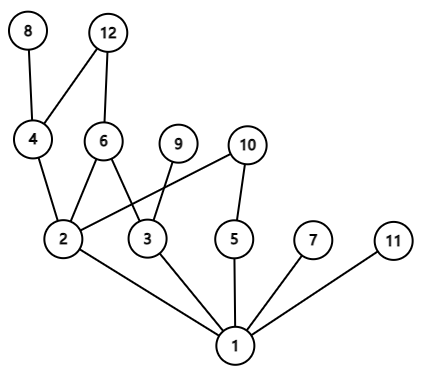
\includegraphics[width=0.4\textwidth]{graph.png}
    }

    令$B_1=\{2,3,6\},B_2=\{2,4,6\},B_3=\{4,8,12\}$,它们的最大元素、最小元素、极大元素、极小元素、上确界、下确界如下表所示:
    \begin{center}
        \begin{tabular}{|c|c|c|c|c|c|c|}
            \hline
            集合&最大元素&最小元素&极大元素&极小元素&上确界&下确界\\
            \hline
            B_1&6&无&\{6\}&\{2,3\}&6&1\\
            \hline
            B_2&无&2&\{4,6\}&\{2\}&12&2\\
            \hline
            B_3&无&4&\{8,12\}&\{4\}&无&4\\
            \hline
        \end{tabular}
    \end{center}
\end{solution}
\paragraph{32.}写出集合$A$及半序关系$\preccurlyeq$的所有元素。
\begin{solution}
    \begin{equation*}
        \begin{aligned}
            A=\{&0,1,2,3,4,5,6\}\\
            \preccurlyeq=\{&(0,1),(0,2),(0,3),(0,4),(0,5),(0,6),(2,5),(3,5),(4,6),\\
            &(0,0),(1,1),(2,2),(3,3),(4,4),(5,5),(6,6)\}
        \end{aligned}
    \end{equation*}
\end{solution}
\paragraph{34.}设$\preccurlyeq_1, \preccurlyeq_2$分别是定义在非空集合$A, B$上半序关系,如下定义$\preccurlyeq_3$:
    \begin{equation*}
        \begin{aligned}
            &\forall a_1,a_2\in A,\ b_1, b_2\in B\\
            &((a_1,b_1),(a_2,b_2))\in\preccurlyeq_3\iff (a_1,a_2)\in\preccurlyeq_1\wedge\ (b_1,b_2)\in\preccurlyeq_2
        \end{aligned}
    \end{equation*}

证明:$\preccurlyeq_3$是$A\times B$上的半序关系。
\begin{proof}

    1.(自反性)设$a\in A,b\in B$,由$\preccurlyeq_1,\preccurlyeq_2$的自反性知
    \begin{equation*}
        (a,a)\in\preccurlyeq_1\wedge\ (b,b)\in\preccurlyeq_2\ \Rightarrow ((a, b), (a, b))\in\preccurlyeq_3
    \end{equation*}

    2.(反对称性)设$a_1,a_2\in A,\ b_1, b_2\in B$,
    \begin{equation*}
        \begin{aligned}
            \text{若有}\ &((a_1,b_1),(a_2,b_2))\in\preccurlyeq_3\wedge\ ((a_2,b_2),(a_1,b_1))\in\preccurlyeq_3\\
            \Rightarrow&(a_1,a_2)\in\preccurlyeq_1\wedge\ (a_2,a_1)\in\preccurlyeq_1\wedge\ (b_1,b_2)\in\preccurlyeq_2\wedge\ (b_2,b_1)\in\preccurlyeq_2\\
            &\text{(由}\preccurlyeq_1,\preccurlyeq_2\text{的反对称性知)}\\
            \Rightarrow&a_1=a_2\wedge b_1=b_2\\
            \Rightarrow&(a_1,b_1)=(a_2,b_2)
        \end{aligned}
    \end{equation*}

    3.(传递性)设$a_1,a_2,a_3\in A,\ b_1,b_2,b_3\in B$,
    \begin{equation*}
        \begin{aligned}
            &((a_1,b_1),(a_2,b_2))\in\preccurlyeq_3\wedge\ ((a_2,b_2), (a_3,b_3))\in\preccurlyeq_3\\
            \Rightarrow&(a_1,a_2)\in\preccurlyeq_1\wedge\ (a_2,a_3)\in\preccurlyeq_1\wedge\ (b_1,b_2)\in\preccurlyeq_2\wedge\ (b_2,b_3)\in\preccurlyeq_2\\
            &\text{(由}\preccurlyeq_1,\preccurlyeq_2\text{的传递性知)}\\
            \Rightarrow&(a_1,a_3)\in\preccurlyeq_1\wedge\ (b_1,b_3)\in\preccurlyeq_2\\
            \Rightarrow&((a_1,b_1), (a_3, b_3))\in \preccurlyeq_3
        \end{aligned}
    \end{equation*}

    综上,$\preccurlyeq_3$满足自反性,反对称性,传递性,则$\preccurlyeq_3$是半序关系。
\end{proof}
\paragraph{36.}
\begin{solution}

令有限集合$A=\{1,2,3,12,18\}$,无限集合$B=\{2^n,3^m,12,18:n,m\in\mathbb{N}\}$,则有关于\textbf{整除关系}的非空半序集合$(A,|),(B,|)$,取$C=\{2,3\}$,则$C$为$A,B$的子集,下面对三问关于$C$分别进行验证。

(1).$C$中没有最大元素。

(2).$C$在$A,B$中都有最大下界$1$,没有最小元素。

(3).$C$在$A,B$中都有上界$\{12,18\}$,没有最小上界。
\end{solution}
\paragraph{习题五}
\paragraph{3.}\begin{solution}

    (1). 单射的,因为$\forall x, y\in \mathbb{N},\ x^2+1=y^2+1\Rightarrow\ x = y$,不是满射,因为$f(x) = 3$无解。

    (2). 满射的,因为$f(0) = 1, f(1) = 0$,不是单射的,因为 $f(0) = f(2) = 1$。

    (3). 既不是单射也不是满射,不是单射,因为$f(0)=f(2)=1$,不是满射,因为$\mathfrak{R}(f) = \{0, 1\} \neq \mathbb{N}$。

    (4). 满射的,因为$\forall m\in \mathbb{N}, f(m, 1) = m$,不是单射,因为$f(2,4)=f(4,2)=16$。

    (5). 双射的,因为$f(x)$是线性函数,由$x = \dfrac{f(x)+17}{3}$知,$f(x)$是单射也是满射。

    (6). 单射的,因为$n = 10^{f(n)}$,不是满射,因为$f(n) = \log_{10}n = -1$,无解。

    (7). 既不是单射也不是满射,不是单射,因为$f(A_1, A_2) = f(A_2, A_1)$,不是满射,因为$f((A_1, A_2)) = (\varnothing, \{X\})$,由于$\{X\}\not\subset \varnothing$,且$A_1\cap A_2\subset A_1\cup A_2$,则不存在这样的$(A_1, A_2)$满足条件。
\end{solution}

\paragraph{6.}设$f$和$g$是函数,$f\subset g$并且$\mathfrak{D}(g)\subset\mathfrak{D}(f)$,证明$f=g$。
\begin{proof}
    由于$f\subset g$,所以只需证$g\subset f$。
    
    对$\forall x\in\mathfrak{D}(g)$,由于$\mathfrak{D}(g)\subset\mathfrak{D}(f)$,则有$x\in\mathfrak{D}(f)$,故$(x,f(x))\in f$。
    
    又由于$f\subset g$,则$(x,f(x))\in g$,于是有$f(x) = g(x)\Rightarrow (x, g(x)) \in f$,故$g\subset f$。

    综上,$f = g$。
\end{proof}

\paragraph{11.}\begin{solution}
    \begin{equation*}
        \begin{aligned}
            p^{-1} = 
            \begin{pmatrix}
                1&2&3\\
                2&3&1
            \end{pmatrix}\\
            p\diamond p^{-1} = 
            \begin{pmatrix}
                1&2&3\\
                1&2&3
            \end{pmatrix}
        \end{aligned}
    \end{equation*}
\end{solution}
\paragraph{12.}设$A$是无限集合,$B$是有限集合。
\begin{solution}

    (1). $A\cap B$不是无限集合,因为$A\cap B\subset B$,而$B$是有限集合,有限集合的子集还是有限集合。

    (2). $A\cup B$是无限集合,因为$A\subset A\cup B$,而$A$是无限集合,包含无限集合的集合一定是无限集合。

    (3). $A\backslash B$是无限集合,因为无限集中去除有限多个元素,仍然是无限集,所以$A\backslash B$是无限集合。
\end{solution}

\end{document}
